\section{Dataset Preparation}
\subsection{Data Sources}
The eC-Tab2Text dataset was constructed using product reviews and specifications extracted from the \href{https://pricebaba.com/}{Pricebaba} website. This source provides detailed information on electronic devices, such as mobile phones and laptops, including expert reviews and structured product attributes. The study focused exclusively on mobile phone data due to the richness of the descriptions and expert evaluations. Each review contained sections on pros and cons and feature-specific details, such as camera performance, battery life, and display quality.

\subsection{Data Extraction and Format}
Data was extracted using web scraping techniques and stored in JSON format to maintain structure and compatibility with modern data processing workflows. Two JSON files were created:
\begin{itemize}
    \item \textbf{Reviews JSON:} Captures attributes like pros, cons, and detailed textual descriptions.
    \item \textbf{Specifications JSON:} Contains key-value pairs for both key specifications and full technical details.
\end{itemize}
Figures \ref{fig:pricebaba-review-structure} and \ref{fig:pricebaba-spec-structure} illustrate the data structures.

\begin{figure}[H]
    \centering
    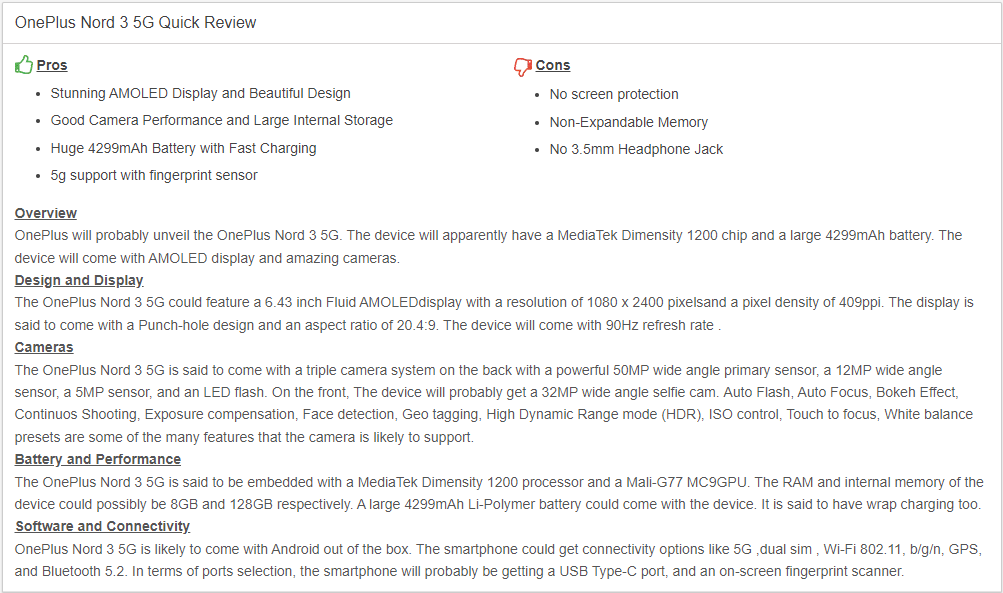
\includegraphics[width=12cm]{images/pricebaba_review_structure.png}
    \caption{pricebaba reviews structure \cite{OnePlusNord35G2023}}
    \label{fig:pricebaba-review-structure}
\end{figure}
\begin{figure}[H]
    \centering
    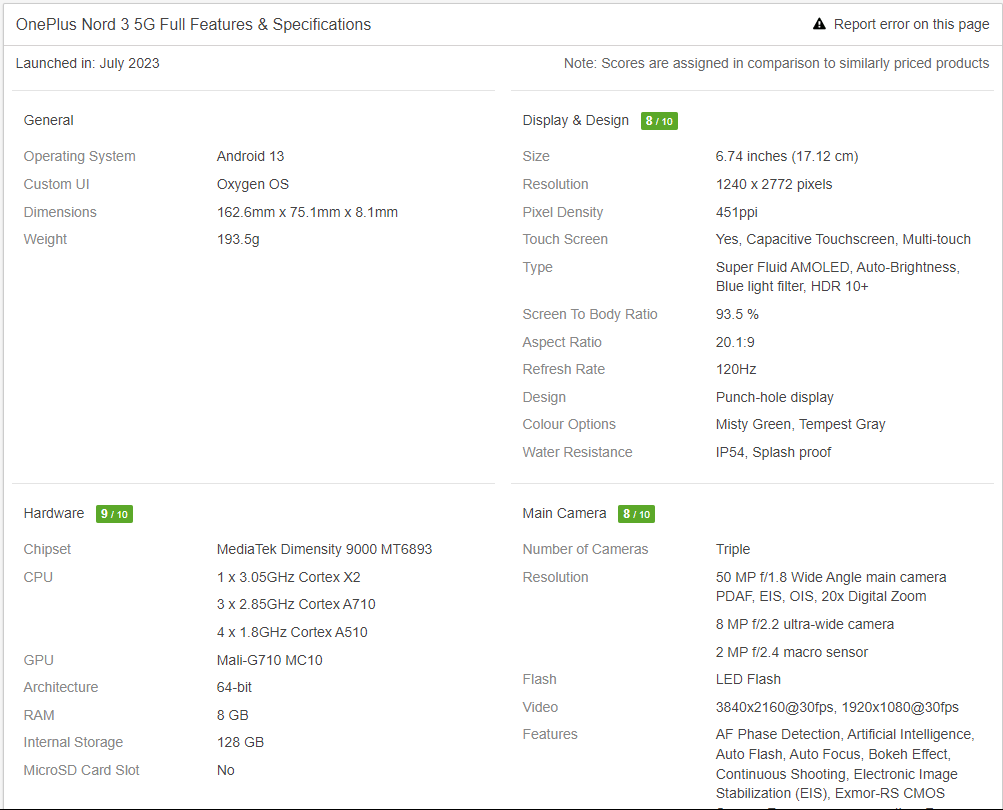
\includegraphics[width=12cm]{images/pricebaba_spec_structure.png}
    \caption{pricebaba specifications structure \cite{OnePlusNord35G2023}}
    \label{fig:pricebaba-spec-structure}
\end{figure}

\subsection{Data Format}
The chosen format for data representation is JSON, as this format allows for structured and easy-to-process data representation. Two JSON files will be used to represent the data: one for the reviews and another for the product specifications. This last one will contains two parts per product: the key values, which means the most important data of the product, and the full specifications. Each JSON file will contain an array of objects, where each object will represent a product along with its respective reviews or specifications. The structure of the JSON files is outlined below:
\newpage
\begin{lstlisting}[style=jsonstyle, frame = single, caption=JSON Data Format Product specification, label=code:json-data-format]
{
    "url": {
        "keys_specifications": [],
        "full_specifications": [
            "Launch Date": "Launch Date",
            "General": {
                "subcategories1": [
                    "value1"
                    ],
                "subcategories2": [
                    "value1",
                    "value2"
                    ],
                ...
            },
            "Characteristic1": {
                "subcategories1": [
                    "value1"
                    ],
                "subcategories2": [
                    "value1",
                    "value2"
                    ],
                ...
            },
            "Characteristic2": {
                "subcategories1": [
                    "value1"
                    ],
                "subcategories2": [
                    "value1",
                    "value2"
                    ],
                ...
            },
            ...
        ]
    },
}
\end{lstlisting}
\newpage
\begin{lstlisting}[style=jsonstyle, frame = single, caption=JSON Data Format reviews, label=code:json-data-format]
{
    "url": {
        "text": {
            "Characteristic1": ["Description1"],
            "Characteristic2": ["Description2"],
            ...
        },
        "Pros": [
            "Pro 1",
            "Pro 2",
            "Pro 3"
        ],
        "Cons": [
            "Con 1",
            "Con 2",
            "Con 3"
        ]
    },
}
\end{lstlisting}

\subsection{Data Cleaning and Normalization}
To ensure consistency and usability, the extracted data underwent rigorous cleaning and normalization:
\begin{itemize}
    \item Standardizing all values to lowercase.
    \item Replacing special characters (e.g., `\&` with `and`).
    \item Reordering keys for logical and contextual coherence.
\end{itemize}
For instance, the key `Display \& Design` was transformed into `Design and Display` to improve readability.

\subsection{Data Integration}
The reviews and specifications JSON files were merged into a unified dataset by matching entries based on their unique product URLs. This ensured that each product's reviews and specifications were consolidated into a single cohesive data entry.

\subsection{Data Filtering}
Irrelevant and redundant entries were removed to refine the dataset further:
\begin{itemize}
    \item Discarding reviews with no textual content in the `text` field.
    \item Removing specifications containing only generic data, such as entries labeled `General`.
    \item Excluding overly simplistic reviews categorized as `Overview`.
\end{itemize}

\subsection{Data Splitting}
The finalized dataset was divided into training and testing sets with an 80\%-20\% split. This ensured a sufficient volume of data for training while retaining a reliable subset for evaluation.

\section{Prompt Structuration}
\subsection{Prompts for Dataset 1 (eC-Tab2Text)}
Prompts were carefully designed to guide models in generating detailed, contextually relevant reviews based on specific product attributes. Each prompt instructed the model to utilize key product features from the JSON-structured data and generate reviews adhering to the given keys. For example, a prompt could ask the model to focus on ``Design and Display'' and ``Battery.'' The dataset was expanded to approximately 12k high-quality prompts through key permutation strategies, facilitating extensive training and evaluation.

For this purpose, instructions with the following structure will be created:
\begin{lstlisting}[style=textstyle, frame = single, caption=Prompt structuration, label=code:prompt-structuration]
"Given following json that contains specifications of a product, generate a review of the key characteristics with json format. Follow the structure on Keys to write the Output: 
### Product: Product for JSON specifications
### Keys: Combination of the keys of the JSON reviews
### Output: reviews for JSON reviews accordingly to the keys"
\end{lstlisting}
it means that instructions will be generated for each permutation of the review keys. For example, if there is a review with the keys Design and Display', Camera', Battery', Performance', Software', i' instructions are chosen from the possible combinations of these keys, where i' is the number of instructions desired to be generated. This approach ensures that the model generates reviews according to the different characteristics of the products. An example of key selection could be that if a product has the keys Design and Display', Camera', Battery', Performance', Software', then the keys Design and Display', Camera' might be selected to generate one instruction, and for another instruction for the same product, the keys Design and Display', Battery' might be selected, and so on.
\\\\
With these combinations of keys for generating instructions, from the original 7,400 data points, 60,700 instructions are obtained that will be used to train the models. These instructions are the final dataset, which is available on \href{https://huggingface.co/datasets/kokujin/json_data_luis}{Hugginface}.

\begin{table}[ht]
    \footnotesize
    \centering
    \begin{tblr}{hline{1,2,Z} = 0.8pt, hline{3-Y} = 0.2pt,
                 colspec = {Q[l,m, 13em] Q[l,m, 6em]},
                 colsep  = 4pt,
                 row{1}  = {0.4cm, font=\bfseries, bg=gray!30},
                 row{2-Z} = {0.1cm},
                 }
    \textbf{Topic}       & \textbf{Value} \\ 
    \SetCell[c=2]{c} \textit{Input}\\
    \# Samples & 11,994\\
    Avg \# Attributes & 59.8\\
    Max \# Attributes & 68\\
    \SetCell[c=2]{c} \textit{Output}\\
    \# Queries & 3354\\
    Avg \# words/query & 56.61\\
    \end{tblr}
\caption{Statistics of eC-Tab2Text dataset}
\label{table:eC-Tab2Text-statistics}
\end{table}

\subsection{Prompts for Dataset 2 (QTSUMM)}
This dataset will be use to applied a cross-validation technique to evaluate the models. The data will be obtained for an existing dataset that is not product-based, but it is focused on structured data in JSON format. The dataset is QTSUMM \cite{zhao2023qtsummqueryfocusedsummarizationtabular}, which contains the columns: table, which contains JSON format data; query, which is the `keys' the model will use to generate the output; and summary, the expected output. The dataset is structured as shown in Figure \ref{fig:qsumm-structure}, where each object contains the columns especified before. This dataset will be used to generate prompts for the models to evaluate their performance.

\begin{figure}[H]
    \centering
    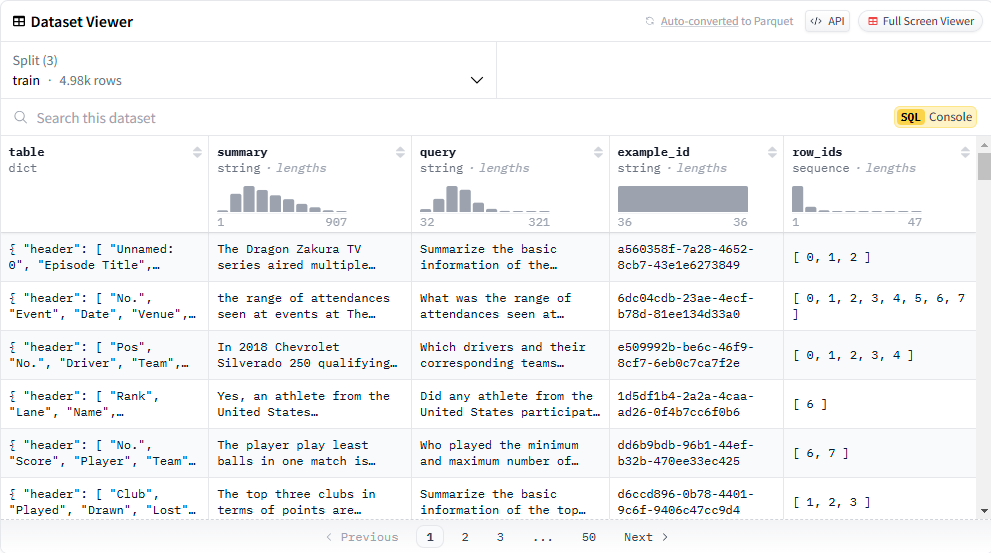
\includegraphics[width=12cm]{images/qsumm_structure.png} 
    \caption{QTSUMM dataset structure \cite{zhao2023qtsummqueryfocusedsummarizationtabular}}
    \label{fig:qsumm-structure}
\end{figure}

For QTSUMM, prompts were structured similarly but adapted to its unique characteristics. The `prompts` column in QTSUMM was filled with data derived from the `table`, `query`, and `summary` columns, ensuring the model understood instructions regardless of the dataset used.

For the QTSUMM dataset, the `prompts' column will be filled with data as follows:
\newpage
\begin{lstlisting}[style=textstyle, frame = single, caption=Prompt structuration, label=code:prompt-structuration]
"Given following json that contains specifications of a product, generate a review of the key characteristics with json format. Follow the structure on Keys to write the Output: 
### Product: Column table of JSON specifications
### Keys: Column query of the dataset
### Output: Column summary of the dataset"
\end{lstlisting}
The `prompt' as shown have the same format for both dataset, but the data used to fill them are different. This will allows the models understands the instructions no matter the dataset used to train or evaluate them.

\section{Model Fine-Tuning}

The eC-Tab2Text dataset provides a diverse and robust set of inputs and outputs, as summarized in Table~\ref{table:eC-Tab2Text-statistics}. The input JSON files contain rich attribute-based product specifications, with an average of 59.8 attributes per product and a maximum of 68 attributes for the most detailed entries. On the output side, the queries are designed to be concise and precise, with an average word count of 22.5 per query, enabling focused evaluation and training of the LLMs.

\subsection{eC-Tab2Text Evaluation} 
\label{sec:evaluation}

\paragraph{Model Fine-Tuning.} To evaluate the effectiveness of the eC-Tab2Text dataset, three state-of-the-art Large Language Models (LLMs) were fine-tuned:

\begin{itemize} 
    \item \textbf{Llama2-chat 7B}: This model is specifically designed for interactive tasks and demonstrates advanced conversational capabilities through fine-tuning on instruction-based datasets \cite{touvron2023llama}. 
    \item \textbf{StructLM 7B}: A pre-trained model optimized for structured text processing and table-to-text generation, StructLM uses a transformer architecture with enhancements for structured data encoding, showcasing its robustness in domain-specific text generation tasks \cite{zhuang2024structlm}. 
    \item \textbf{Mistral\_Instruct 7B}: Known for its high adaptability, this model leverages supervised fine-tuning with diverse instruction-following datasets, achieving state-of-the-art performance in multi-modal and domain-adapted text generation \cite{jiang2023mistral}. 
\end{itemize}

The fine-tuning process involved training the models with eC-Tab2Text's curated dataset to assess their capabilities in generating high-quality, contextually accurate outputs tailored to e-commerce applications. By aligning with studies emphasizing the importance of instruction tuning and domain-specific dataset alignment to enhance LLM performance \cite{Zhang2023InstructionTF, Chang2023ASO}, the models were configured with parameters optimized for computational efficiency, as detailed in Table~\ref{table:hyperparameters}. The fine-tuning focused on adapting the models to handle the domain-specific tasks of generating detailed and attribute-focused product reviews.

\begin{table}[ht]
    \centering
    \footnotesize
    \begin{tabular}{|c|c|}
    \hline
    \textbf{Hyperparameter} & \textbf{Value} \\
    \hline
    Learning Rate & $2 \times 10^{-4}$ \\
    Batch Size & 2 \\
    Epochs & 1 \\
    Gradient Accumulation Steps & 1 \\
    Weight Decay & 0.001 \\
    Max Sequence Length & 900 \\
    \hline
    \end{tabular}
    \caption{Hyperparameter settings for fine-tuning.}
    \label{table:hyperparameters}
\end{table}

Furthermore, the `BitsAndBytesConfig` library from Hugging Face's `transformers` has been utilized for model optimization. These additional hyperparameters are shown in Table \ref{table:hyperparameters-bitsandbytes}.
\begin{table}[H]
    \centering
    \begin{tabular}{|c|c|}
        \hline
        \textbf{Hyperparameter} & \textbf{Value} \\
        \hline
        bnb\_4bit\_compute\_dtype & float16 \\
        bnb\_4bit\_quant\_type & nf4 \\
        use\_nested\_quant & False \\
        \hline
    \end{tabular}
    \caption{Hyperparameters Selection BitsAndBytes}
    \label{table:hyperparameters-bitsandbytes}
\end{table}

\paragraph{Metrics.} Evaluation metrics are essential for assessing the quality of text generation models. The most widely used metrics include: 

\begin{itemize} 
    \item \textbf{BLEU (Bilingual Evaluation Understudy)} \cite{Papineni02bleu:a}: Commonly used in machine translation and natural language generation, BLEU measures the overlap of n-grams between generated and reference texts. Despite its popularity, BLEU has limitations, particularly in capturing semantic similarity and evaluating beyond exact matches \cite{Reiter2018A}. 
    \item \textbf{ROUGE (Recall-Oriented Understudy for Gisting Evaluation)} \cite{lin-2004-rouge}: Focuses on recall-oriented evaluation by comparing the overlap of n-grams, word sequences, and word pairs between generated summaries and reference texts. It is highly effective for summarization tasks \cite{Ganesan2015ROUGE}.
    \item \textbf{METEOR (Metric for Evaluation of Translation with Explicit ORdering)}\cite{10.5555/1626355.1626389}: Incorporates stemming, synonymy, and flexible matching, providing a more nuanced evaluation than BLEU. It strongly correlates with human judgments, especially in translation tasks \cite{Dobre2015ACB}. 
    \item \textbf{BERTScore} \cite{zhang2020bertscoreevaluatingtextgeneration}: Leverages contextual embeddings from pre-trained transformer models to measure semantic similarity between generated and reference texts. Unlike n-gram-based metrics, BERTScore captures meaning and context, offering a robust evaluation for text generation tasks \cite{zhang2020bertscoreevaluatingtextgeneration}.
\end{itemize}

\paragraph{Prometheus Evaluation (Hallucination)} 
\label{appendix:Prometheus}

To evaluate model-based metrics, the Prometheus framework \cite{kim2024prometheus2opensource} was employed, utilizing structured prompts for three key evaluation criteria: fluency, correctness, and faithfulness \footnote{https://github.com/prometheus-eval/prometheus-eval}. The primary framework leverages an Absolute System Prompt, which defines the role of the evaluator and ensures objective, consistent assessments based on established rubrics. This Absolute System Prompt, shown in Listing\ref{code:ABS-System-Prompt}, forms the foundation for all evaluations across metrics.

\begin{lstlisting}[style=textstyle, frame = single, caption=Absolute System Prompt \cite{kim2024prometheus2opensource}, label=code:ABS-System-Prompt]
You are a fair judge assistant tasked with providing clear, objective feedback based on specific criteria, ensuring each assessment reflects the absolute standards set for performance.
\end{lstlisting}
The task descriptions for evaluating fluency, correctness, and faithfulness share a similar structure, as shown in Listing\ref{code:Task-description-Faithfulness},\ref{code:Task-description-fluency-correctness}. These instructions define the evaluation process, requiring detailed feedback and a score between 1 and 5, strictly adhering to a given rubric.

\vspace{15pt}

\begin{lstlisting}[style=textstyle, frame = single, caption=Task description used for evaluation of faithfulness \cite{kim2024prometheus2opensource}, label=code:Task-description-Faithfulness]
###Task Description:
An instruction (might include an Input inside it), a response to evaluate, a reference answer that gets a score of 5, and a score rubric representing a evaluation criteria are given.
1. Write a detailed feedback that assess the quality of the response strictly based on the given score rubric, not evaluating in general.
2. After writing a feedback, write a score that is an integer between 1 and 5. You should refer to the score rubric.
3. The output format should look as follows: "Feedback: (write a feedback for criteria) [RESULT] (an integer number between 1 and 5)"
4. Please do not generate any other opening, closing, and explanations.
5. Only evaluate on common things between generated answer and reference answer. Don't evaluate on things which are present in reference answer but not in generated answer.
\end{lstlisting}

\begin{lstlisting}[style=textstyle, frame = single, caption=Task description used for evaluation of fluency and correctness \cite{kim2024prometheus2opensource}, label=code:Task-description-fluency-correctness]
###Task Description:
An instruction (might include an Input inside it), a response to evaluate, a reference answer that gets a score of 5, and a score rubric representing a evaluation criteria are given.
1. Write a detailed feedback that assess the quality of the response strictly based on the given score rubric, not evaluating in general.
2. After writing a feedback, write a score that is an integer between 1 and 5. You should refer to the score rubric.
3. The output format should look as follows: "Feedback: (write a feedback for criteria) [RESULT] (an integer number between 1 and 5)"
4. Please do not generate any other opening, closing, and explanations.
\end{lstlisting}

\paragraph{Instructions for Evaluation}

Prometheus prompts are customized for each evaluation metric. Below are the specialized structures and rubrics for fluency, faithfulness, and correctness.

\paragraph{Faithfulness}
This metric ensures the generated response aligns with both the provided context and reference answers. The evaluation structure incorporates specific rubrics for relevance and information consistency.

\begin{lstlisting}[style=textstyle, frame = single, caption=Prompt structured correctness \cite{kim2024prometheus2opensource}, label=code:estructured-faithfulness]
###The instruction to evaluate:
Evaluate the fluency of the generated JSON answer.
###Context:
{Prompt}
###Existing answer (Score 5):
{reference_answer}
###Generate answer to evaluate:
{response}
###Score Rubrics:
"score1_description":"If the generated answer is not matching with any of the reference answers and also not having information from the context.",
"score2_description":"If the generated answer is having information from the context but not from existing answer and also have some irrelevant information.",
"score3_description":"If the generated answer is having relevant information from the context and some information from existing answer but have additional information that do not exist in context and also do not in existing answer.",
"score4_description":"If the generated answer is having relevant information from the context and some information from existing answer.",
"score5_description":"If the generated answer is matching with the existing answer and also having information from the context."}
###Feedback:
\end{lstlisting}

\paragraph{Fluency}
This metric evaluates the grammatical accuracy and readability of the generated response.

\begin{lstlisting}[style=textstyle, frame = single, caption=Prompt structured fluency \cite{kim2024prometheus2opensource}, label=code:estructured-fluency]
###The instruction to evaluate: Evaluate 
the fluency of the generated JSON answer
###Response to evaluate: {response}
###Reference Answer (Score 5): 
{reference_answer}
###Score Rubrics:
"score1_description":"The generated JSON answer is not fluent and is difficult to understand.",
"score2_description":"The generated JSON answer has several grammatical errors and awkward phrasing.",
"score3_description":"The generated JSON answer is mostly fluent but contains some grammatical errors or awkward phrasing.",
"score4_description":"The generated JSON answer is fluent with minor grammatical errors or awkward phrasing.",
"score5_description":"The generated JSON answer is perfectly fluent with no grammatical errors or awkward phrase
###Feedback:
\end{lstlisting}

\paragraph{Correctness}
This metric assesses the logical accuracy and coherence of the generated response compared to the reference.

\begin{lstlisting}[style=textstyle, frame = single, caption=Prompt estructured correctness \cite{kim2024prometheus2opensource}, label=code:estructured-correctness]
###The instruction to evaluate:
Your task is to evaluate the generated answer and reference answer for the query: {Prompt}
###Response to evaluate:
{response}
###Reference Answer (Score 5):
{reference_answer}
###Score Rubrics:
"criteria": "Is the model proficient in generate a coherence response",
"score1_description": "If the generated answer is not matching with any of the reference answers.",
"score2_description": "If the generated answer is according to reference answer but not relevant to user query.",
"score3_description": "If the generated answer is relevant to the user query and reference answer but contains mistakes.",
"score4_description": "If the generated answer is relevant to the user query and has the exact same metrics as the reference answer, but it is not as concise.",
"score5_description": "If the generated answer is relevant to the user query and fully correct according to the reference answer.

###Feedback: 
\end{lstlisting}

\paragraph{Cross-Validation.} Performed to validate the robustness and generalizability of the fine-tuned models by testing them across distinct datasets. This process ensured the models could adapt effectively to different structured data scenarios while maintaining high performance. Specifically, the same three models fine-tuned on the eC-Tab2Text dataset (\textbf{Llama2-chat 7B}, \textbf{StructLM 7B}, and \textbf{Mistral\_Instruct 7B}) were trained and evaluated on the QTSumm dataset \cite{zhao2023qtsummqueryfocusedsummarizationtabular}, using identical hyperparameters as detailed in Section~\ref{sec:evaluation}.
\paragraph{\textit{QTSumm Dataset.}\label{par:Prompt QTSumm}\cite{zhao2023qtsummqueryfocusedsummarizationtabular}} Designed for query-focused summarization tasks, it includes structured JSON data, queries, and summaries. This dataset provided an ideal contrast to eC-Tab2Text, as its focus lies on general-purpose summarization rather than product-specific reviews. The models were trained using prompts structured similarly to those used with the eC-Tab2Text dataset. The key distinction in the QTSumm setup was the row-level content included in the prompts, as outlined in \ref{code:Prompt Dataset 2}. This alignment ensured training consistency while leveraging the QTSumm dataset's unique characteristics.

\begin{lstlisting}[style=textstyle, frame = single, caption=Prompt structuration for QTSumm, label=code:Prompt Dataset 2]
    "Given following json that contains specifications of a product, generate a review of the key characteristics with json format. Follow the structure on Keys to write the Output: 
    ### Product: Column table of JSON specifications
    ### Keys: Column query of the dataset
    ### Output: Column summary of the dataset"
    \end{lstlisting}

\section{Resume}
This section provides a detailed overview of the methodology used for generating product reviews on e-commerce platforms using Large Language Models (LLMs). It describes the entire process from data collection and preparation, where data was generated from scratch, meticulously cleaned, and structured for further processing.
\\\\
The section continues by detailing the model tuning techniques, including the selection of hyperparameters and optimization methods, tailored to match the computational limits of the hardware. This phase was essential for adapting the models to produce relevant product reviews. The effectiveness of these fine-tuned models was then measured using evaluation metrics such as BLEU, METEOR, and ROUGE to assess the quality of generated reviews against actual product reviews.